
\documentclass[xcolor=dvipsnames]{beamer}  % for hardcopy add 'trans'

\mode<presentation>
{
  \usetheme{Singapore}
  % or ...
  \setbeamercovered{transparent}
  % or whatever (possibly just delete it)
}

\usefonttheme{professionalfonts}
\usepackage[russian]{babel}
% or whatever
%\usepackage[latin1]{inputenc}
% or whatever
%\usepackage{times}
%\usepackage[T1]{fontenc}
% Or whatever. Note that the encoding and the font should match. If T1
% does not look nice, try deleting the line with the fontenc.

%%%%%%%%%%%%%%%%%%%%%% start my preamble %%%%%%%%%%%%%%%%%%%%%%


\addtobeamertemplate{navigation symbols}{}{%
    \usebeamerfont{footline}%
    \usebeamercolor[fg]{footline}%
    \hspace{1em}%
    \insertframenumber/\inserttotalframenumber
} 

\setbeamercolor{footline}{fg=blue}
\setbeamerfont{footline}{series=\bfseries}


%\usepackage{epsfig}
\usepackage{graphicx}
\graphicspath{{./figs_code/}}

\usepackage{amsmath, amssymb, amsthm}

\usepackage{fancyvrb}

\usepackage{tikz}
\usetikzlibrary{arrows}
\usetikzlibrary{calc}
\usetikzlibrary{intersections}
\usetikzlibrary{decorations}
\usepackage{pgf}
\usepackage{pgfplots}
\pgfplotsset{compat=1.13}

\usepackage{graphviz}
 
\usepackage{verbatim}


\usepackage{algorithmicx,algpseudocode}


%font
\usepackage{mathpazo}
%\usepackage[usenames, dvipsnames]{color}

%\usepackage[linesnumbered, ruled, lined]{algorithm2e}

\usepackage{xr}
\externaldocument[ET-]{et}


\newcommand*{\theorembreak}{\usebeamertemplate{theorem end}\framebreak\usebeamertemplate{theorem begin}}

\newcommand{\newtopic}[1]{\textcolor{Green}{\Large \bf #1}}
\newcommand{\navy}[1]{\textcolor{Blue}{\bf #1}}
\newcommand{\navymth}[1]{\textcolor{Blue}{#1}}
\newcommand{\red}[1]{\textcolor{red}{#1}}


\definecolor{pale}{RGB}{235, 235, 235}
\definecolor{pale2}{RGB}{175,238,238}
\definecolor{turquois4}{RGB}{0,134,139}

% Typesetting code
\definecolor{bg}{rgb}{0.95,0.95,0.95}
\usepackage{minted}
\usemintedstyle{friendly}
\newminted{python}{mathescape,frame=lines,framesep=4mm,bgcolor=bg}
\newminted{ipython}{mathescape,frame=lines,framesep=4mm,bgcolor=bg}
\newminted{julia}{mathescape,frame=lines,framesep=4mm,bgcolor=bg}
\newminted{c}{mathescape,linenos=true}
\newminted{r}{mathescape,  frame=none, baselinestretch=1, framesep=2mm}
\renewcommand{\theFancyVerbLine}{\sffamily
    \textcolor[rgb]{0.5,0.5,1.0}{\scriptsize {\arabic{FancyVerbLine}}}}


\usepackage{stmaryrd}

\newcommand{\Fact}{\textcolor{Brown}{\bf Факт. }}
\newcommand{\Facts}{\textcolor{Brown}{\bf Факты }}
\newcommand{\keya}{\textcolor{turquois4}{\bf Ключевая идея. }}
\newcommand{\Factnodot}{\textcolor{Brown}{\bf Факт }}
\newcommand{\Eg}{\textcolor{ForestGreen}{Пример. }}
\newcommand{\Egs}{\textcolor{ForestGreen}{Примеры. }}
\newcommand{\Ex}{{\bf Ex. }}
\newcommand{\Thm}{\textcolor{Brown}{\bf Теорема. }}
\newcommand{\Prf}{\textcolor{turquois4}{\bf Доказательство. }}
\newcommand{\Ass}{\textcolor{turquois4}{\bf Допущение.}} 
\newcommand{\Lem}{\textcolor{Brown}{\bf Лемма. }}

%source code 



% cali
\usepackage{mathrsfs}
\usepackage{bbm}
\usepackage{subfigure}

\newcommand{\argmax}{\operatornamewithlimits{argmax}}
\newcommand{\argmin}{\operatornamewithlimits{argmin}}

\newcommand\T{{\mathpalette\raiseT\intercal}}
\newcommand\raiseT[2]{\raisebox{0.25ex}{$#1#2$}}

\DeclareMathOperator{\cl}{cl}
%\DeclareMathOperator{\argmax}{argmax}
\DeclareMathOperator{\interior}{int}
\DeclareMathOperator{\Prob}{Prob}
\DeclareMathOperator{\kernel}{ker}
\DeclareMathOperator{\diag}{diag}
\DeclareMathOperator{\sgn}{sgn}
\DeclareMathOperator{\determinant}{det}
\DeclareMathOperator{\trace}{trace}
\DeclareMathOperator{\Span}{span}
\DeclareMathOperator{\rank}{rank}
\DeclareMathOperator{\cov}{cov}
\DeclareMathOperator{\corr}{corr}
\DeclareMathOperator{\range}{rng}
\DeclareMathOperator{\var}{var}
\DeclareMathOperator{\mse}{mse}
\DeclareMathOperator{\se}{se}
\DeclareMathOperator{\row}{row}
\DeclareMathOperator{\col}{col}
\DeclareMathOperator{\dimension}{dim}
\DeclareMathOperator{\fracpart}{frac}
\DeclareMathOperator{\proj}{proj}
\DeclareMathOperator{\colspace}{colspace}

\providecommand{\inner}[1]{\left\langle{#1}\right\rangle}

% mics short cuts and symbols
% mics short cuts and symbols
\newcommand{\st}{\ensuremath{\ \mathrm{s.t.}\ }}
\newcommand{\setntn}[2]{ \{ #1 : #2 \} }
\newcommand{\cf}[1]{ \lstinline|#1| }
\newcommand{\otms}[1]{ \leftidx{^\circ}{#1}}

\newcommand{\fore}{\therefore \quad}
\newcommand{\tod}{\stackrel { d } {\to} }
\newcommand{\tow}{\stackrel { w } {\to} }
\newcommand{\toprob}{\stackrel { p } {\to} }
\newcommand{\toms}{\stackrel { ms } {\to} }
\newcommand{\eqdist}{\stackrel {\textrm{ \scriptsize{d} }} {=} }
\newcommand{\iidsim}{\stackrel {\textrm{ {\sc iid }}} {\sim} }
\newcommand{\1}{\mathbbm 1}
\newcommand{\dee}{\,{\rm d}}
\newcommand{\given}{\, | \,}
\newcommand{\la}{\langle}
\newcommand{\ra}{\rangle}

\renewcommand{\rho}{\varrho}

\newcommand{\htau}{ \hat \tau }
\newcommand{\hgamma}{ \hat \gamma }

\newcommand{\boldx}{ {\mathbf x} }
\newcommand{\boldu}{ {\mathbf u} }
\newcommand{\boldv}{ {\mathbf v} }
\newcommand{\boldw}{ {\mathbf w} }
\newcommand{\boldy}{ {\mathbf y} }
\newcommand{\boldb}{ {\mathbf b} }
\newcommand{\bolda}{ {\mathbf a} }
\newcommand{\boldc}{ {\mathbf c} }
\newcommand{\boldi}{ {\mathbf i} }
\newcommand{\bolde}{ {\mathbf e} }
\newcommand{\boldp}{ {\mathbf p} }
\newcommand{\boldq}{ {\mathbf q} }
\newcommand{\bolds}{ {\mathbf s} }
\newcommand{\boldt}{ {\mathbf t} }
\newcommand{\boldz}{ {\mathbf z} }

\newcommand{\boldzero}{ {\mathbf 0} }
\newcommand{\boldone}{ {\mathbf 1} }

\newcommand{\boldalpha}{ {\boldsymbol \alpha} }
\newcommand{\boldbeta}{ {\boldsymbol \beta} }
\newcommand{\boldgamma}{ {\boldsymbol \gamma} }
\newcommand{\boldtheta}{ {\boldsymbol \theta} }
\newcommand{\boldxi}{ {\boldsymbol \xi} }
\newcommand{\boldtau}{ {\boldsymbol \tau} }
\newcommand{\boldepsilon}{ {\boldsymbol \epsilon} }
\newcommand{\boldmu}{ {\boldsymbol \mu} }
\newcommand{\boldSigma}{ {\boldsymbol \Sigma} }
\newcommand{\boldOmega}{ {\boldsymbol \Omega} }
\newcommand{\boldPhi}{ {\boldsymbol \Phi} }
\newcommand{\boldLambda}{ {\boldsymbol \Lambda} }
\newcommand{\boldphi}{ {\boldsymbol \phi} }

\newcommand{\Sigmax}{ {\boldsymbol \Sigma_{\boldx}}}
\newcommand{\Sigmau}{ {\boldsymbol \Sigma_{\boldu}}}
\newcommand{\Sigmaxinv}{ {\boldsymbol \Sigma_{\boldx}^{-1}}}
\newcommand{\Sigmav}{ {\boldsymbol \Sigma_{\boldv \boldv}}}

\newcommand{\hboldx}{ \hat {\mathbf x} }
\newcommand{\hboldy}{ \hat {\mathbf y} }
\newcommand{\hboldb}{ \hat {\mathbf b} }
\newcommand{\hboldu}{ \hat {\mathbf u} }
\newcommand{\hboldtheta}{ \hat {\boldsymbol \theta} }
\newcommand{\hboldtau}{ \hat {\boldsymbol \tau} }
\newcommand{\hboldmu}{ \hat {\boldsymbol \mu} }
\newcommand{\hboldbeta}{ \hat {\boldsymbol \beta} }
\newcommand{\hboldgamma}{ \hat {\boldsymbol \gamma} }
\newcommand{\hboldSigma}{ \hat {\boldsymbol \Sigma} }

\newcommand{\boldA}{\mathbf A}
\newcommand{\boldB}{\mathbf B}
\newcommand{\boldC}{\mathbf C}
\newcommand{\boldD}{\mathbf D}
\newcommand{\boldI}{\mathbf I}
\newcommand{\boldL}{\mathbf L}
\newcommand{\boldM}{\mathbf M}
\newcommand{\boldP}{\mathbf P}
\newcommand{\boldQ}{\mathbf Q}
\newcommand{\boldR}{\mathbf R}
\newcommand{\boldX}{\mathbf X}
\newcommand{\boldU}{\mathbf U}
\newcommand{\boldV}{\mathbf V}
\newcommand{\boldW}{\mathbf W}
\newcommand{\boldY}{\mathbf Y}
\newcommand{\boldZ}{\mathbf Z}

\newcommand{\bSigmaX}{ {\boldsymbol \Sigma_{\hboldbeta}} }
\newcommand{\hbSigmaX}{ \mathbf{\hat \Sigma_{\hboldbeta}} }

\newcommand{\RR}{\mathbbm R}
\newcommand{\CC}{\mathbbm C}
\newcommand{\NN}{\mathbbm N}
\newcommand{\PP}{\mathbbm P}
\newcommand{\EE}{\mathbbm E \nobreak\hspace{.1em}}
\newcommand{\EEP}{\mathbbm E_P \nobreak\hspace{.1em}}
\newcommand{\ZZ}{\mathbbm Z}
\newcommand{\QQ}{\mathbbm Q}


\newcommand{\XX}{\mathcal X}

\newcommand{\aA}{\mathcal A}
\newcommand{\fF}{\mathscr F}
\newcommand{\bB}{\mathscr B}
\newcommand{\iI}{\mathscr I}
\newcommand{\rR}{\mathscr R}
\newcommand{\dD}{\mathcal D}
\newcommand{\lL}{\mathcal L}
\newcommand{\llL}{\mathcal{H}_{\ell}}
\newcommand{\gG}{\mathcal G}
\newcommand{\hH}{\mathcal H}
\newcommand{\nN}{\textrm{\sc n}}
\newcommand{\lN}{\textrm{\sc ln}}
\newcommand{\pP}{\mathscr P}
\newcommand{\qQ}{\mathscr Q}
\newcommand{\xX}{\mathcal X}

\newcommand{\ddD}{\mathscr D}


\newcommand{\R}{{\texttt R}}
\newcommand{\risk}{\mathcal R}
\newcommand{\Remp}{R_{{\rm emp}}}

\newcommand*\diff{\mathop{}\!\mathrm{d}}
\newcommand{\ess}{ \textrm{{\sc ess}} }
\newcommand{\tss}{ \textrm{{\sc tss}} }
\newcommand{\rss}{ \textrm{{\sc rss}} }
\newcommand{\rssr}{ \textrm{{\sc rssr}} }
\newcommand{\ussr}{ \textrm{{\sc ussr}} }
\newcommand{\zdata}{\mathbf{z}_{\mathcal D}}
\newcommand{\Pdata}{P_{\mathcal D}}
\newcommand{\Pdatatheta}{P^{\mathcal D}_{\theta}}
\newcommand{\Zdata}{Z_{\mathcal D}}


\newcommand{\e}[1]{\mathbbm{E}[{#1}]}
\newcommand{\p}[1]{\mathbbm{P}({#1})}

%\theoremstyle{plain}
%\newtheorem{axiom}{Axiom}[section]
%\newtheorem{theorem}{Theorem}[section]
%\newtheorem{corollary}{Corollary}[section]
%\newtheorem{lemma}{Lemma}[section]
%\newtheorem{proposition}{Proposition}[section]
%
%\theoremstyle{definition}
%\newtheorem{definition}{Definition}[section]
%\newtheorem{example}{Example}[section]
%\newtheorem{remark}{Remark}[section]
%\newtheorem{notation}{Notation}[section]
%\newtheorem{assumption}{Assumption}[section]
%\newtheorem{condition}{Condition}[section]
%\newtheorem{exercise}{Ex.}[section]
%\newtheorem{fact}{Fact}[section]

% Bibliography
\usepackage[authordate,uniquename=false,firstinits,backend=biber,maxcitenames=2]{biblatex-chicago}
\DeclareFieldFormat[article]{title}{#1}
\DeclareFieldFormat[inproceedings]{title}{#1}
\addbibresource{et_newbib.bib}
\renewcommand{\cite}{\textcite}



\setlength{\parskip}{1.5ex plus0.5ex minus0.5ex}


\setlength{\jot}{12pt} 









\title{A Primer in Econometric Theory}

\subtitle
{Lecture 9: Confidence Intervals and Tests}

\author{John Stachurski \\ \tiny Lectures by Akshay Shanker}




\begin{document}

\begin{frame}
  \titlepage
\end{frame}


\begin{frame}
    
    \vspace{2em}
    Focus till now has been on point estimation
    
    Data are not
    infinite --- point estimation involves uncertainty
    
    \vspace{.7em}
    In this lecture:
    \begin{itemize}
        \item quantify estimation uncertainty using the language
    of confidence sets
        \item cover hypothesis tests, which are a second key
    method of inference in classical statistics
    \end{itemize}
\end{frame}


\begin{frame}
    
    \vspace{2em}
    We'll work with parametric
    language
    
    Similar notation as previously in Ch. 8, except:
    %
    \begin{enumerate}
        \item the marginal distribution $P$ of each observation $\boldz_n$ is
            written as $P_{\theta}$
        \item the universe $\pP$ of possible distributions is
            $\setntn{P_{\theta}}{\theta \in \Theta}$
        \item the joint distribution of the data $\zdata = (\boldz_1,
            \ldots, \boldz_N)$ is written as $\Pdatatheta$
    \end{enumerate}
    
    \vspace{.7em}
    Not restricting ourselves to the case of finitely many
    parameters
    
    \begin{itemize}
        \item think of $\theta$ as an index
        over the set of distributions
    \end{itemize}

\end{frame}

\section{Confidence Sets}

\begin{frame}\frametitle{Confidence Sets}
    
    \vspace{2em}
    Confidence sets are random subsets of model space that contain the true data
    generating process with high probability
    
\end{frame}

\begin{frame}\frametitle{Finite Sample Confidence Sets}

    \vspace{2em}
    Fix $\alpha \in (0,1)$
    
    A random set $C(\zdata) \subset \Theta$ 
    is called a \navy{$1 - \alpha$ confidence set} for $\theta$ if
    $C(\zdata)$ is observable given the data and, for any $\theta \in
    \Theta$,
    %
    \begin{equation*}
        \label{eq:proci}
        \PP \{ \theta  \in C(\zdata) \} \geq 1 - \alpha
        \quad \text{whenever} \quad
        \lL(\zdata) = \Pdatatheta
    \end{equation*}
    
    \vspace{.7em}
    Note that it's the set that's random here, not $\theta$
        
\end{frame}

\begin{frame}

    \vspace{2em}
    Suppose we want to estimate the mean of an unknown
    distribution based on a set of observations $\zdata$
    
    \vspace{.7em}
    A 95\% confidence set $C(\zdata)$ will
    contain the mean in about 95\% of our experiments, \emph{regardless of the 
    underlying distribution}
    
    \vspace{.7em}
    We don't know what $\theta$ is, and so
    the set \emph{must be designed} such that the probability of containing
    $\theta$ exceeds $1 - \alpha$ regardless of which $\theta$ is generating the
    data
    
\end{frame}

\begin{frame}

    \vspace{2em}
    The difficulty is to actually construct a confidence set with this
    property for a reasonably large class of distributions
    
    A traditional approach that uses strong parametric assumptions:

    \vspace{.7em}
    \Eg
    Let $\zdata = \boldx = (x_1,\ldots,x_N)$ where each $x_n$ is an
    independent draw from $\nN(\mu, \sigma^2)$
    
    Suppose for now that 
    only $\mu \in \RR$ is unknown
    
    We wish to form a confidence
    interval for $\mu$.  Since $\lL(\bar x_N) 
        = \nN \left(\mu, \, \frac{\sigma^2}{N} \right)$, we have
    %
    \begin{equation}
        \label{eq:cisk}
        \lL \left[
            \sqrt N \frac{(\bar x_N - \mu)}{\sigma}  
        \right]
        = \nN(0, 1)
    \end{equation}
    
\end{frame}

\begin{frame}
    
    \vspace{2em}
    \Eg (cont.)
    Above statement true regardless of the values of $\mu$ and
    $\sigma$
    
    Recall that if $\lL(x) = F$, $x$ has a symmetric density and $F$
    is strictly increasing, then 
    %
    \begin{equation*}
    \label{eq:symcdf}
        c = F^{-1}(1 - \alpha/2) 
        \quad \implies \quad
        \PP\{-c \leq x \leq c\} = 1 - \alpha
    \end{equation*}

    As such, 
    %
    \begin{equation*}
        \PP
            \left\{ 
            \frac{\sqrt{N}}{\sigma} | \bar x_N - \mu | 
            \leq z_{\alpha/2}
            \right\}
        = 1 - \alpha
    \end{equation*}
    $\quad \text{when} \quad
        z_{\alpha/2} := \Phi^{-1} \left(1 - \frac{\alpha}{2} \right)$
        
    Here $\Phi$ is the standard normal {\sc cdf}

\end{frame}

\begin{frame}

    \vspace{2em}
    \Eg (cont.)
    Rearranging the above gives
    %
    \begin{equation*}
        \PP
            \left\{ 
            \bar x_N - 
                \frac{\sigma}{\sqrt{N}} z_{\alpha/2}
            \leq \mu \leq 
            \bar x_N + 
                \frac{\sigma}{\sqrt{N}} z_{\alpha/2}
            \right\}
        = 1 - \alpha
    \end{equation*}

    The above argument is true regardless of the value of $\mu$. We then conclude
    %
    \begin{equation*}
        C(\boldx) 
        := (\bar x_N - e_n, \, \bar x_N + e_n)
        \quad \text{with} \quad
        e_n := \frac{\sigma}{\sqrt{N}} z_{\alpha/2}
    \end{equation*}
    %
    is a $1 - \alpha$ confidence interval for $\mu$. (Note that
    $C(\boldx)$ is indeed observable under our assumption that $\sigma$ is known.)
    
\end{frame}

\begin{frame}

    \vspace{2em}
    In the above example, assumption that $\sigma$ is known is clearly
    unrealistic
    
    If $\sigma$ is unknown,  replace the
    term with the sample standard deviation $s_N$. In doing so, we will use the following fact
    
    \vspace{.7em}
    \Fact\eqref{ET-fa:ctdr}
        If $x_1,\ldots,x_N$ are {\sc iid} draws from $\nN(\mu, \sigma^2)$, then
        %
        \begin{equation}
            \label{eq:cisk2}
            \sqrt{N - 1} \frac{(\bar x_N - \mu)}{s_N} 
        \end{equation}
        %
        has a Student's $t$-distribution with $N-1$ degrees of freedom
    
    \vspace{.7em}    
    The random variable \eqref{eq:cisk2} is called a \navy{pivot}, its distribution
    does not depend on the unknown parameters
    
\end{frame}

\begin{frame}

    \vspace{2em}
    \Eg
    Continue with setting of the previous example
    
    Recall $\zdata = \boldx = (x_1,\ldots,x_N)$ where each $x_n$ is an
    independent draw from $\nN(\mu, \sigma^2)$
    
    Now let both $\sigma$ and $\mu$ be unknown 
    
    \vspace{.7em}
    Let $F_{N-1}$ be the {\sc cdf} of the $t$-distribution with
    $N-1$ degrees of freedom.  Using the same reasoning as in the
    above example, with $z_{\alpha/2}$ replaced by $t_{\alpha/2} :=
    F^{-1}_{N-1}(1 - \alpha/2)$, we obtain
    %
    \begin{equation*}
        \PP 
            \left\{ 
            \bar x_N - 
                \frac{s_N}{\sqrt{N-1}} t_{\alpha/2}
            \leq \mu \leq 
            \bar x_N + 
                \frac{s_N}{\sqrt{N-1}} t_{\alpha/2}
            \right\}
        = 1 - \alpha
    \end{equation*}
    
\end{frame}

\begin{frame}
    
    \vspace{2em}
    Recall that the standard deviation of $\bar x_N$ is $\sigma/ \sqrt{N}$
    
    The term $s_N/\sqrt{N-1}$ is a sample estimate of $\sigma/ \sqrt{N}$
    
    Call $s_N/\sqrt{N-1}$ 
    the standard error of
    $\bar x_N$ and write it as $\se(\bar x_N)$
    
    \vspace{.7em}
    Now write the confidence
    interval for $\mu$ in the previous example as
    %
    \begin{equation}
        \label{eq:citc}
        C(\boldx) := (\bar x_N - \se(\bar x_N) t_{\alpha/2},\;
             \bar x_N + \se(\bar x_N) t_{\alpha/2})
    \end{equation}


\end{frame}

\begin{frame}\frametitle{Asymptotic Methods}

    \vspace{2em}
    Given $\alpha \in (0,1)$, a set
    $C_N(\zdata) \subset \Theta$ is called an \navy{asymptotic $1 - \alpha$
    confidence set} for $\theta$ if $C_N(\zdata)$ is observable given
    the data and
    %
    \begin{equation*}
        \label{eq:procia}
        \lim_{N \to \infty} \PP \{ \theta \in C_N(\zdata)  \} \geq 1 - \alpha
    \end{equation*}
    
    for all $\theta \in \Theta$
    
    \vspace{.7em}
    Note $C_N(\zdata)$ is a
    sequence of sets and the definition concerns this sequence
    
\end{frame}

\begin{frame}

    \vspace{2em}
    Consider first the case
    of scalar $\theta$
    
    Suppose we have an estimator $\hat \theta_N$ of $\theta$
    that is asymptotically normal for all $\theta \in \Theta$
    
    \vspace{.7em}
    For all $\theta
    \in \Theta$, there exists a positive constant $v(\theta)$ such that
    %
    \begin{equation}
        \label{eq:asnorm2}
        \sqrt{N} (\hat \theta_N - \theta) \tod \nN(0, v(\theta)) 
            \quad \text{as} \quad
            N \to \infty
    \end{equation}
    
    (Recall results in  \S\ref{ET-sss:ad} where we discuss asymptotic properties of estimators and specialise to the scalar case)
    
\end{frame}

\begin{frame}

    \vspace{2em}
    The constant $v(\theta)$ is called the asymptotic variance 
    of $\hat \theta_N$
    
    \vspace{.7em}
    Suppose we have a sequence of statistics $\se(\hat \theta_N)$
    such that
    %
    \begin{equation}
        \label{eq:secfs}
        \sqrt{N} \se(\hat \theta_N)
            \toprob \sqrt{v(\theta)} 
            \quad \text{as} \quad
            N \to \infty
    \end{equation}
    %
    Next, \eqref{eq:asnorm2} and
    \eqref{eq:secfs} imply 
    %
    \begin{equation}
        \label{eq:nbsez}
        \frac{\hat \theta_N - \theta}{\se(\hat \theta_N)} 
        \, \tod \, \nN(0, 1)
        \quad \text{as} \quad
        N \to \infty
    \end{equation}
    
    (Exercise~\ref{ET-ex:nbsez})
    

\end{frame}

\begin{frame}

    \vspace{2em}
    We can now create our asymptotic confidence intervals as
    %
    \begin{equation*}
        \label{eq:sacine}
        C_N := 
        (\hat \theta_N - \se(\hat \theta_N) z_{\alpha/2}, 
        \, \hat \theta_N + \se(\hat \theta_N) z_{\alpha/2})
    \end{equation*}
    
    To see this, take the limit and apply \eqref{eq:nbsez} to get
    %
    \begin{align*}
        \lim_{N \to \infty} \PP \{ \theta \in C_N(\zdata) \} 
        & = \lim_{N \to \infty} 
            \PP
                \{ 
                \hat \theta_N - 
                    \se(\hat \theta_N) z_{\alpha/2}
                \leq \theta \leq 
                \hat \theta_N \\
        &\quad + \se(\hat \theta_N) z_{\alpha/2}
                    \} \\
        & = \lim_{N \to \infty} 
            \PP 
                \left\{ 
                    -z_{\alpha/2}
                    \leq \frac{\hat \theta_N - \theta}{\se(\hat \theta_N)}
                    \leq z_{\alpha/2}
                \right\} \\
        & = 1 - \alpha
    \end{align*}
    
\end{frame}

\begin{frame}
    
    \vspace{2em}
    \Eg
    Let $\bar x_N$ be the sample mean of {\sc iid} data $\{x_n\}$
    
    Suppose that these data come from some distribution with finite second
    moment
    
    Let $\mu$ denote the common mean and let $\sigma^2$ denote the
    variance
    
    Let $s_N$ be the sample standard deviation
\end{frame}

\begin{frame}

    \vspace{2em}
    \Eg (cont.)
    Combine the
    central limit theorem and consistency of $s_N$ for $\sigma$ (see
    page~\pageref{ET-eg:ssdc}):
    %
    \begin{align*}
        \label{eq:smnse}
        \sqrt{N}(\bar x_N - \mu) \tod \nN(0, \sigma^2)
        \;  \text{ and } \;
        \sqrt{N}\se(\bar x_N) \toprob \sigma
        \quad  \\ \text{for} \quad
        \se(\bar x_N) := \frac{s_N}{\sqrt{N}}
    \end{align*}
    
    \vspace{.7em}
    With this definition of $\se(\bar x_N)$,
    the set
    %
    \begin{equation*}
        (\bar x_N - \se(\bar x_N) z_{\alpha/2}, 
            \, \bar x_N + \se(\bar x_N) z_{\alpha/2})
    \end{equation*}
    %
    is an asymptotic $1-\alpha$ confidence interval for $\bar x_N$
\end{frame}

\begin{frame}\frametitle{Non-Parametric Example}
    
    \vspace{2em}
    In \S\ref{ET-ss:eds} of ET we learned that if $\boldx = (x_1, \ldots, x_N)$ is a vector
    of {\sc iid} draws from some {\sc cdf} $F$ and $\hat F_N$ is the corresponding
    {\sc ecdf},  then $ \| F - \hat F_N \|_{\infty}$ converges in probability to
    $0$
    
    \vspace{.7em}
    In 1933, A.\ N.\ Kolmogorov used an extension of the central limit theorem
    to obtain an asymptotic distribution for this term
    

\end{frame}

\begin{frame}

    \vspace{2em}
    In particular, he showed
    that when $F$ is continuous,
    
    \begin{equation}
    \label{eq:kr}
    \sqrt{N} \sup_{s \in \RR} |\hat F_N(s) - F(s)| \tod K
    \end{equation}
    %
    where $K$ is the \navy{Kolmogorov} {\sc cdf}
    %
    \begin{equation*}
        K(s) := \frac{\sqrt{2 \pi}}{s} \sum_{i=1}^{\infty}
        \exp \left[ - \frac{(2 i - 1)^2 \pi^2}{8 s^2} \right]
        \qquad (s \geq 0)
    \end{equation*}
\end{frame}

\begin{frame}

    \vspace{2em}
    As in the CLT, the limiting distribution $K$ is independent of the
    {\sc cdf} $F$ that generates the data
    
    We can use Kolmogorov's result, Equation \eqref{eq:kr}, to produce an asymptotic $1-\alpha$ \
    confidence set for $F$
    
    \vspace{.7em}
    Let $\mathfrak F$ be the set of all {\sc cdf}s  on $\RR$, let
    $x_1,\ldots,x_N$ be {\sc iid} draws from $F \in \mathfrak F$,
    let $k_{1-\alpha} := K^{-1}(1 - \alpha)$, and let
    %
    \begin{multline*}
        C_N(\boldx) := \bigg\{ G \in \mathfrak F
            \; : \; \hat F_N(s) - \frac{k_{1-\alpha}}{\sqrt{N}} \leq G(s) \leq 
            \hat F_N(s) \\ +  \frac{k_{1-\alpha}}{\sqrt{N}} \; \text{ for all } \; s \in \RR \bigg\}
    \end{multline*}
    
\end{frame}

\begin{frame}

    \vspace{2em}
    The set $C_N(\boldx) \subset \mathfrak F$ is an asymptotic $1-\alpha$
    confidence set for $F$
    
    Indeed, after rearranging the expression, we get
    %
    \begingroup
    \addtolength{\jot}{1em}
    \begin{align*}
        F \in C_N(\boldx) 
        & \iff  - k_{1-\alpha} \leq \sqrt{N}(\hat F_N(s) - F(s)) \leq k_{1-\alpha}
        \; \text{ for all } \; s  \\
        & \iff  \sqrt{N}|\hat F_N(s) - F(s)| \leq k_{1-\alpha}
        \; \text{ for all } \; s  \\
        & \iff  \sup_s \sqrt{N}|\hat F_N(s) - F(s)| \leq k_{1-\alpha} 
    \end{align*}
    \endgroup
    
\end{frame}

\begin{frame}
    
    \vspace{2em}
    Apply \eqref{eq:kr} to confirm our claim:
    %
    \begin{align*}
        & \lim_{N \to \infty} \PP \{ F \in C_N(\boldx) \}\\
        & = \lim_{N \to \infty} \PP 
         \left\{ \sup_s \sqrt{N}|\hat F_N(s) - F(s)| \leq k_{1-\alpha} \right\}\\
        & = 1 - \alpha
    \end{align*}
    
    
\end{frame}

\begin{frame}
    
    \vspace{2em}
    Present the confidence set $C_N(\boldx)$ visually:
    
    \begin{itemize}
        \item highlighting the
    area between the lower bound $\hat F_N(s) - k_{1-\alpha}/\sqrt{N}$ and the
    upper bound $\hat F_N(s) + k_{1-\alpha}/\sqrt{N}$ over $s$
    \end{itemize}
   
   \vspace{.7em}
    Consider data  drawn from a
    $t$-distribution $F$ with 10 degrees of freedom and $\alpha$ is set to $0.05$...

\end{frame}

\begin{frame}

    \begin{figure}
    \centering
    \scalebox{.44}{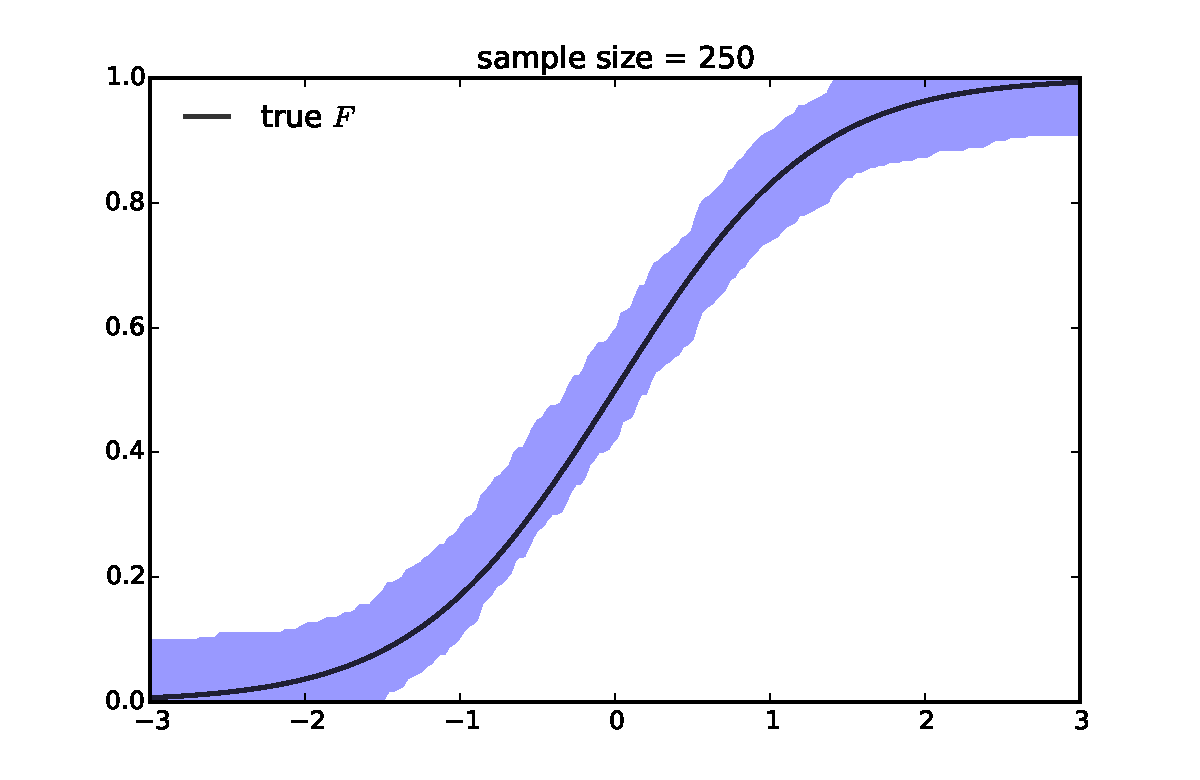
\includegraphics[trim={0em 0em 0em 0em}, clip]{ks_sim1.pdf}}
    \caption{\label{f:ks_sim1} Confidence set for the {\sc ecdf} with 250 observations}
    \end{figure}

\end{frame}

\begin{frame}

    \begin{figure}
    \centering
    \scalebox{.44}{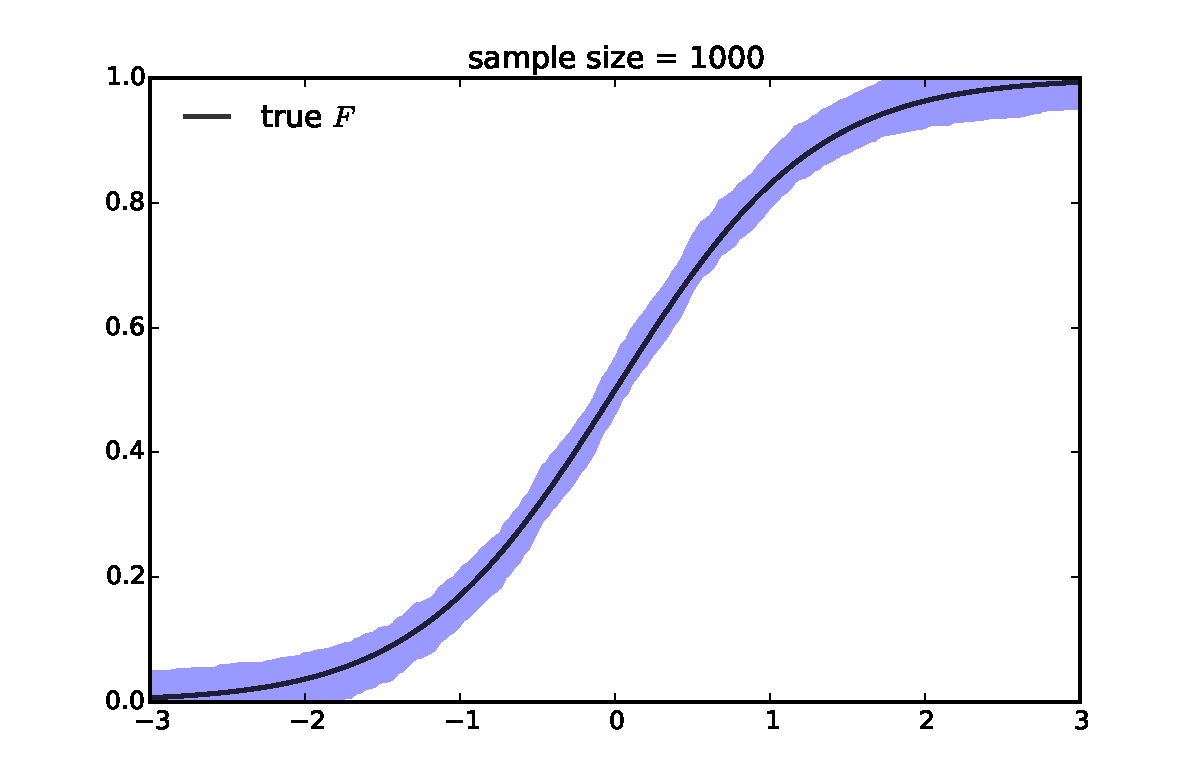
\includegraphics[trim={0em 0em 0em 0em}, clip]{ks_sim2.pdf}}
    \caption{\label{f:ks_sim2} Confidence set for the {\sc ecdf} with 1,000 observations}
    \end{figure}
    
\end{frame}

\section{Hypothesis Tests}

\begin{frame}\frametitle{Hypothesis Testing}
    
    \vspace{2em}
    This section considers problems of inference where we
    %
    \begin{enumerate}
        \item hold a belief or theory concerning the probabilities generating the
            data and
        \item consider whether the data provides evidence for or against that theory
    \end{enumerate}
    
\end{frame}

\begin{frame}

    \vspace{2em}
    \Eg
    Asset price returns data tend to have heavier tails than the
    normal distribution
    
    For certain assets, normality might still be a
    reasonable and convenient approximation
    
    Let's look at whether or not normality provides a reasonable fit in the
    case of daily returns on the Nikkei 225
\end{frame}

\begin{frame}

    \begin{figure}
    \centering
    \scalebox{.4}{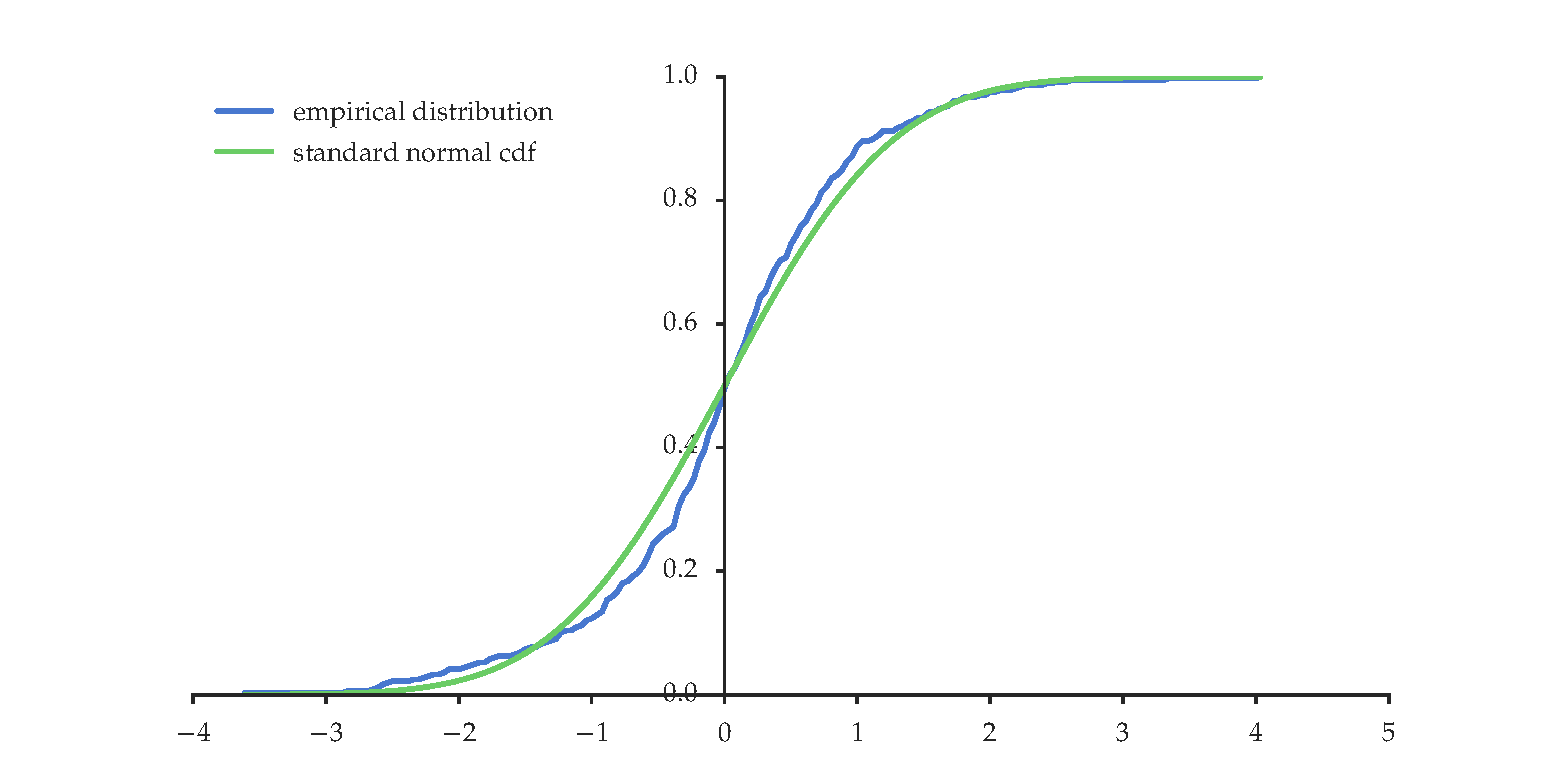
\includegraphics[trim={2em 2em 2em 2em}, clip]{nikkei_ecdf.pdf}}
    \caption{\label{f:nikkei_ecdf} {\sc ECDF} for standardized returns versus the
    standard normal {\sc cdf}}
    \end{figure}

\end{frame}

\begin{frame}
    
    \vspace{2em}
    While the
     {\sc ecdf} of the data and the {\sc cdf} are not identical, we wouldn't
     expect this even if the hypothesis of normality is completely true
     
     \vspace{.7em}
     Question: is the sample ``unlikely" given the
     hypothesis of normality?  

\end{frame}

\begin{frame}\frametitle{Null Hypothesis}

    \vspace{2em}
    Hypothesis testing begins with a \navy{null hypothesis}:
    \begin{itemize}
        \item a statement that the observed data are being generated by a certain
    model, or one of a certain class of models
    \end{itemize}
    
    \vspace{.7em}
    A hypothesis test is an attempt to reject the
    null
    
\end{frame}

\begin{frame}
    
    \vspace{2em}
    Black Swan Karl Popper (1902--1994):
    \begin{itemize}
        \item  claim: \emph{all} swans are white
        \item   no
    quantity of white swan sightings can confirm the claim 
        \item  a single
    black swan can show the claim to be false
    \end{itemize}
    
    \vspace{.7em}
    Attempting to
    falsify a theory on the basis of observation is more
    constructive than attempting to confirm it
    
    Reject the null hypothesis only if strong
    evidence against it is observed -- we
    don't want to mistakenly discard a good theory

\end{frame}

\begin{frame}\frametitle{Constructing Tests}
    
    \vspace{2em}
    We will use notation we used to discuss confidence intervals
    
    A null hypothesis is
    a specification of a set of models that we believe the data-generating process
    belongs to
    
    This amounts to specifying a subset $\Theta_0$ of $\Theta$
    
    The
    null hypothesis often written as 
    %
    \begin{equation*}
        H_0 \colon \theta \in \Theta_0
    \end{equation*}
    %
\end{frame}

\begin{frame}
    
    \vspace{2em}
    If $\Theta_0$ is a singleton, then the null
    hypothesis called a \navy{simple hypothesis}
    
    \vspace{.7em}
    If not, then the null
    hypothesis called a \navy{composite hypothesis}

    \vspace{.7em}
    A test of the null hypothesis is a test of whether or not observed data
    generated by $P_{\theta}$ for some $\theta \in \Theta_0$

\end{frame}

\begin{frame}

    \vspace{2em}
    \Eg
    The hypothesis of purchasing power parity is tested by considering models
    such as 
    %
    \begin{equation*}
        \label{eq:ppp}
        p = a + \beta e p^* + \sigma u   
    \end{equation*}
    %
    where $p$ is a price or index of domestic
    prices, $e$ is an exchange rate, $p^*$ is a corresponding foreign price,
    $u$ is a disturbance term and $a, \beta, \sigma$ are parameters
    
    \vspace{.7em}
    The null
    hypothesis for absolute purchasing power parity is that \eqref{eq:ppp}
    holds with $a = 0$ and
    $\beta=1$
    
    Since $\sigma$ is not pinned down by the null, this is a
    composite null hypothesis
    
\end{frame}

\begin{frame}\frametitle{Rejection Region}

    \vspace{2em}
    Formally, a \navy{test} of $H_0$ is a binary function $\phi$ mapping the
    observed data $\zdata$ into $\{0,1\}$
    
    \vspace{.7em}
    The decision rule:
    %
    \begin{align*}
        \text{if } \phi(\zdata) & = 1, \text{ then reject } H_0   \\
        \text{if } \phi(\zdata) & = 0, \text{ then do not reject } H_0   
    \end{align*}
    %
    (Failing to reject $H_0$ should not be confused with accepting $H_0$.  More on
    this below.) 
    
    Our aim will be to design $\phi$ such that it takes the value $1$ when the
    data present strong evidence against $H_0$
    
\end{frame}

\begin{frame}

    \vspace{2em}
    \Eg
    Let $\zdata$ be a set of pairs $\boldz_n = (x_n, y_n)$ from some unknown
    bivariate distribution $P_{\theta}$
    
    If $H_0$ is the hypothesis that the
    correlation between $x$ and $y$ is negative, then 
    a large positive sample correlation would constitute evidence against $H_0$
    
    Hence our test might take the form $\phi(\zdata) = \1\{\hat \rho >
    c\}$, where $\hat \rho$ is the sample correlation
    
    An appropriate value
    of $c$ remains to be determined 
    
    
\end{frame}

\begin{frame}\frametitle{Type I and Type II error}

    \vspace{2em}
    Two different ways in
    which the realization of \emph{random} $\zdata$ can mislead us
    
    \begin{enumerate}
        \item mistakenly reject the null
    hypothesis when it is in fact true ---  \navy{type I error}
        \item fail to reject the null hypothesis when it is false --- \navy{type II error}
    \end{enumerate}
    
\end{frame}

\begin{frame}

    \vspace{2em}
    The \navy{power function} associated with the test $\phi$ is the function
    %
    \begin{equation*}
        \beta(\theta) := \PP_{\theta} \{\phi(\zdata) = 1\}
        \qquad (\theta \in \Theta)
    \end{equation*}
    
    \vspace{.7em}
    The symbol $\PP_{\theta}$ indicates we are computing
    probabilities under the assumption that $\lL(\zdata) =
    \Pdatatheta$
    \begin{itemize}
        \item $\beta(\theta)$ is the probability the test 
        rejects when the data are generated by the 
        probabilistic model identified by $\theta$
    \end{itemize}
    
    \vspace{.7em}
    Ideally, $\beta(\theta) = 0$ when $\theta \in \Theta_0$, and
    $\beta(\theta) = 1$ when $\theta \notin \Theta_0$ --- in practice,
    difficult to achieve

\end{frame}

\begin{frame}

    \vspace{2em}
    We want to be conservative in rejecting the
    null
    \begin{itemize}
        \item traditional to keep the probability of type I error small 
    \end{itemize}
    
    \vspace{.7em}
    Standard procedure is to choose a small number $\alpha$ such as
    0.05 or 0.01, and then adjust the test such that
    %
    \begin{equation}
        \label{eq:defsize}
        \beta(\theta) \leq \alpha
        \quad \text{for all } \theta \in \Theta_0
    \end{equation}
    
    If (\ref{eq:defsize}) holds, then the test is said to be of \navy{size $\alpha$}
\end{frame}


\begin{frame}
    
    \vspace{2em}
    The \navy{size} of any test with power function $\beta$ is
    %
    \begin{equation*}
        \label{eq:defsize2*}
        \alpha := \sup_{\theta \in \Theta_0} \beta(\theta) 
    \end{equation*}
    %
    This is the maximal rejection probability when the null hypothesis is true
    
\end{frame}


\begin{frame}\frametitle{Critical Values and Tests}

    \vspace{2em}
    In constructing tests, common to 
    define a real-valued \navy{test
    statistic} $T$ and a \navy{critical value} $c$, and then
    set 
    %
    \begin{equation}
        \label{eq:tfftc}
        \phi(\zdata) := \1\{T(\zdata) > c\}
    \end{equation}
    %
    The pair $(T, c)$ then defines the test, and the rule becomes: 
    %
    \begin{equation*}
        \text{reject $H_0$ if and only if } T(\zdata) > c 
    \end{equation*}
    
\end{frame}

\begin{frame}

    \vspace{2em}
    \Eg
    Suppose  $x_1,\ldots,x_N$ are independent draws from $\nN(\mu, 1)$
    where the value of $\mu$ is unknown
    
    The null hypothesis is $\mu
    \leq 0$, or $\Theta_0 = (-\infty, 0]$
    
    Since we want to make inference
    about the mean, a natural choice for our test statistic is the sample
    mean.  Thus 
    %
    \begin{equation*}
        T(\zdata) :=: T(x_1,\ldots,x_N) := \bar x_N 
    \end{equation*}
    %
    Each $c \in \RR$ gives a test via (\ref{eq:tfftc}) on the previous 
    slide, with power function $\beta(\mu) = \PP_{\mu} \{ \bar{x}_N > c\}$
    
\end{frame}

\begin{frame}

    \vspace{2em}
    \Eg(cont.)
    To evaluate
    $\beta$, recall $\lL(\bar{x}_N) = \nN(\mu, 1/N)$
    
    As a result, if
    $\Phi$ is the {\sc cdf} of the standard normal distribution and
    $\lL(z) = \Phi$, then
    %
    \begin{align*}
        \PP_{\mu} \{ \bar{x}_N \leq c \} 
        & = \PP\{ \mu + N^{-1/2} z  \leq c \}\\
        & = \PP\{ z \leq N^{1/2}(c - \mu) \} 
        = \Phi[N^{1/2}(c - \mu)]
    \end{align*}
    %
    \begin{equation}
        \label{eq:pfct}
        \fore
        \beta(\mu) = 1 - \Phi[N^{1/2}(c - \mu)]
    \end{equation}
    
    Given $c$, the power function is increasing in $\mu$ because higher $\mu$
    pushes up the mean of $\bar{x}_N$, making the event $\{ \bar{x}_N > c\}$
    more likely
    
    Given $\mu$, the function is decreasing in $c$, because
    higher $c$ makes the event $\{ \bar{x}_N > c\}$ less likely
    
\end{frame}

\begin{frame}

    \vspace{2em}
    Plots of the power function $\beta$ in \eqref{eq:pfct} 
    \begin{itemize}
        \item two different values of $c$
        \item $N$ is fixed at 10.
        \item  since $\Theta_0 = (-\infty, 0]$, the size of the test in each case is
                $\sup_{\mu \leq 0} \beta(\mu)$. Since the power curves are increasing,
                this is just $\beta(0)$
    \end{itemize}
    
    Typical trade-off between type I and type
    II error. If we increase $c$,
    \begin{itemize}
        \item  we make rejection less likely for all values of
                $\mu$
        \item push down type I error, but also increase the probability
            we fail to reject a false null
    \end{itemize} 

\end{frame}

\begin{frame}

    \begin{figure}
   \begin{center}
    \scalebox{.35}{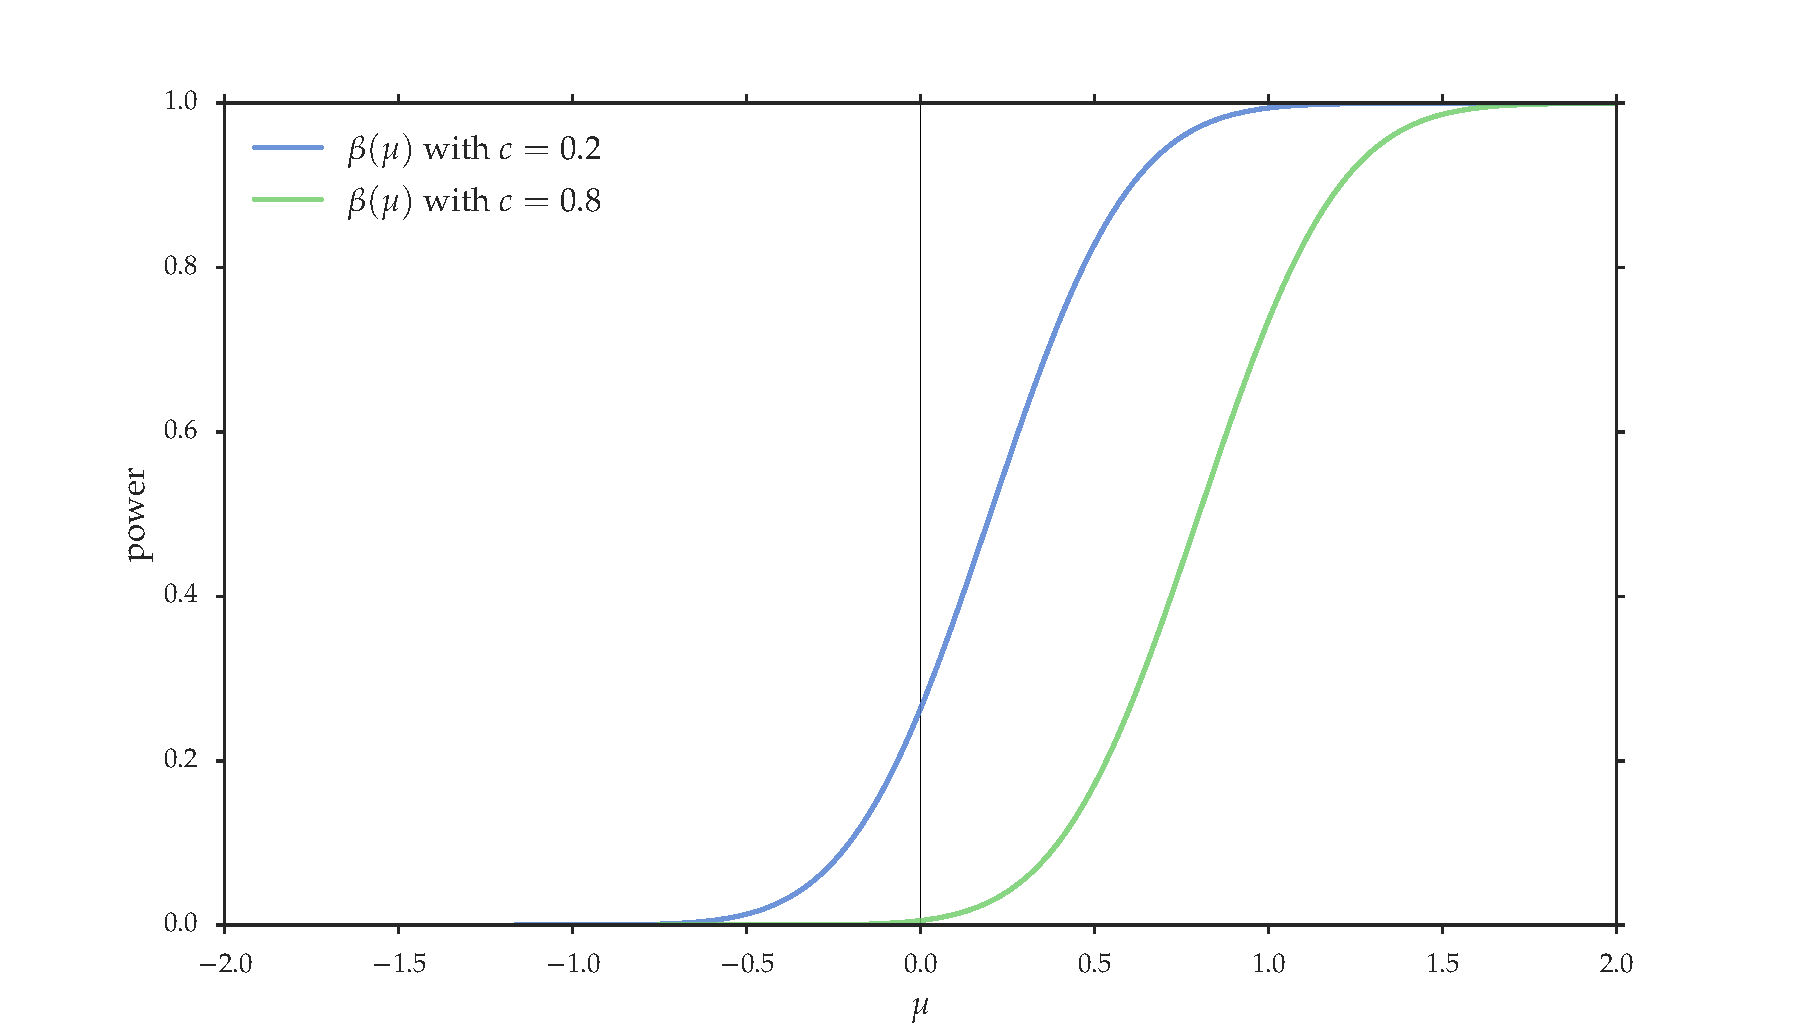
\includegraphics{power.pdf}}
    \caption{\label{f:power} Power function $\beta$}
   \end{center}
    \end{figure}
    
\end{frame}

\begin{frame}\frametitle{Choosing Critical Values}
 
    \vspace{2em}
    Typically, the
    choice of test statistic $T$ suggested by the problem
    \begin{itemize}
        \item example: if our hypothesis is
        a statement about the second moment of a random variable, then take
        $T$ to be the sample second moment
    \end{itemize}
    
    Once $T$ is fixed, we need to adjust the critical region $c$
    such that $(T,c)$ attains the appropriate size
    
    Standard procedure:
    %
    \begin{enumerate}
        \item choose a desired size $\alpha$ according to our tolerance for
        type I error
        \item identify a suitable test statistic $T$
        \item choose a critical value $c$ so that $(T,c)$ is of size $\alpha$
    \end{enumerate}
    
\end{frame}

\begin{frame}

    \vspace{2em}
    In performing the last step, balance our desire to minimize type II
    error while maintaining a size $\alpha$ --- choose $c$ to solve
    %
    \begin{equation}
        \alpha = \sup_{\theta \in \Theta_0} \PP_{\theta}\{T(\zdata) > c\}
    \end{equation}
    
    \vspace{.7em}
    Figure on next slide:
    \begin{itemize}
        \item $\Theta_0=\{\theta_a, \theta_b\}$
        \item  blue line is distribution of $T(\zdata)$ (density) 
                when $\zdata$ generated by $\theta_a$
        \item  black line is the same for
                $\theta_b$
        \item choose $c$ such that the largest of the two shaded
            areas is equal to $\alpha$
    \end{itemize}
    
\end{frame}

\begin{frame}
    
    \begin{figure}
       \begin{center}
        \scalebox{.5}{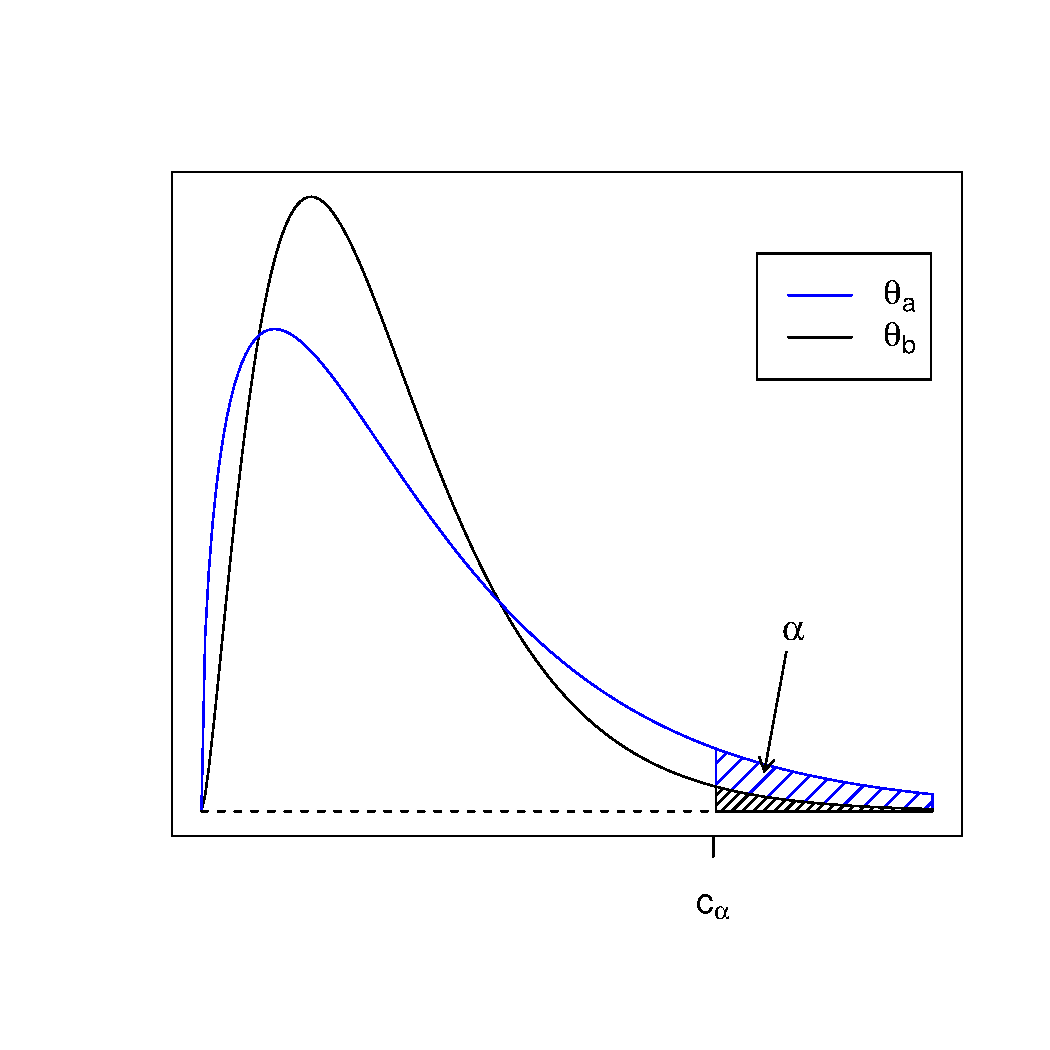
\includegraphics[trim={4em 4em 0em 4em}, clip]{c_alpha.pdf}}
        \caption{\label{f:c_alpha} Determining the critical value}
       \end{center}
    \end{figure}


\end{frame}

\begin{frame}

    \vspace{2em}
    \Eg
    Consider again the previous example. Recall $x_1,\ldots,x_N
    \iidsim \nN(\mu, 1)$ for $\mu$ unknown, and our null hypothesis is
    $\mu \leq 0$
    
    Given $\alpha$, our task is to find the appropriate critical
    value $c$ so that the test $(T,c)$ is of size $\alpha$
    
    \vspace{.7em}
    To solve for $c$ given $\alpha$, we choose $c$ to solve 
    %
    \begin{equation}
        \label{eq:solfc}
        \alpha = \sup_{\theta \in \Theta_0} \PP_{\theta}\{T(\zdata) > c\}
    \end{equation}
    
    Recall the expression for the power function for this setting that
    we calculated in the previous example
    %
    \begin{equation}
    \beta(\mu) = 1 - \Phi[N^{1/2}(c - \mu)]
    \end{equation}
    
\end{frame}

\begin{frame}
    
    \vspace{2em}
    \Eg (cont.)
    We then choose $c$ to solve 
    %
    \begin{equation*}
        \alpha = \sup_{\mu \leq 0} \{ 1 - \Phi[N^{1/2}(c - \mu)] \}
    \end{equation*}
    %
    The right-hand side is increasing in $\mu$, so the supremum is obtained
    by setting $\mu = 0$
    
    Setting $\mu = 0$ and solving for $c$, we
    obtain
    %
    \begin{equation*}
        c(\alpha) := N^{-1/2} \Phi^{-1} (1 - \alpha)
    \end{equation*}
    %
    where $\Phi^{-1}$ is the quantile function of the standard normal
    distribution

\end{frame}

\begin{frame}

    \vspace{2em}
    \Eg (cont.) 
    
    Since $\Phi^{-1}$ is increasing:
    %
    \begin{itemize}
        \item smaller $\alpha$ corresponds to
                larger $c(\alpha)$ --- we reduce the probability of type I error by
                increasing the critical value the mean $\bar{x}_N$ must obtain for
                rejection to occur
        \item higher $N$ brings down $c(\alpha)$, without increasing the probability
                of rejecting a true null
    \end{itemize}
    
\end{frame}

\begin{frame}\frametitle{Asymptotic Tests}

    \vspace{2em}
    In many cases, we know little about the distribution of the test
    statistic
    
     One approach is to determine the asymptotic distribution of the test statistic
     \begin{itemize}
         \item CLT: pin down distributions without actually assuming a
                parametric structure
     \end{itemize}
     
\end{frame}

\begin{frame}

    \vspace{2em}
    Notation $\beta_N$ emphasizes that the power function depends on sample size
    
    A test is
    called \navy{asymptotically of size $\alpha$} if
    %
    \begin{equation*}
        \label{eq:asmposa}
        \lim_{N \to \infty}
        \beta_N(\theta) \leq \alpha
        \quad \text{for all } \theta \in \Theta_0
    \end{equation*}
    
\end{frame}

\begin{frame}\frametitle{Test for the Empirical Distribution}

    \vspace{2em}
    Return to the data on standardized daily
    returns on the Nikkei 225
    
    \vspace{.7em}
    Let $\Phi$ be
    the standard normal {\sc cdf} as before
    
    Let $H_0$ be that standardized
    returns are {\sc iid} draws from $\Phi$
    
    Let $\alpha$ be given, and let
    $k_{1-\alpha} = K^{-1}(1-\alpha)$ be the $1-\alpha$ quantile of the Kolmogorov
    distribution $K$: 
    %
    \begin{equation*}
    K(s) := \frac{\sqrt{2 \pi}}{s} \sum_{i=1}^{\infty}
    \exp \left[ - \frac{(2 i - 1)^2 \pi^2}{8 s^2} \right]
    \qquad (s \geq 0)
    \end{equation*}

    Finally, let $\hat F_N$ be the
    {\sc ecdf} of the data
    
\end{frame}

\begin{frame}
    
    \vspace{2em}
    If the null hypothesis is true, then
    %
    \begin{equation}
        \label{eq:kr2}
        \sqrt{N} \sup_{s \in \RR} |\hat F_N(s) - \Phi(s)| \tod K
    \end{equation}
    %
    For the test
    %
    \begin{equation*}
        \phi_N(\boldx) 
        := \1 \left\{ 
               \sqrt{N} \sup_{s \in \RR} |\hat F_N(s) - \Phi(s)| > k_{1-\alpha}
            \right\}
    \end{equation*}
    %
    let $\beta_N(\Phi)$ be the value of the power function when the null hypothesis is
    true. By \eqref{eq:kr2},
    %
    \begin{equation*}
        \lim_{N \to \infty} \beta_N(\Phi) 
        = \lim_{N \to \infty} 
            \PP \left\{ 
                \sqrt{N}\sup_{s \in \RR} |\hat F_N(s) - \Phi(s)| > k_{1-\alpha}
            \right\}
        = \alpha
    \end{equation*}
    %
    And the test is asymptotically of size
    $\alpha$
    
\end{frame}

\begin{frame}

    \vspace{2em}
    The Nikkei data set used here has 364 observations
    
    The value of the test statistic
    $\sqrt{N}\sup_{s \in \RR} |\hat F_N(s) - \Phi(s)|$ is 1.548
    
    If $\alpha =
    0.05$, then the critical value $k_{1-\alpha}$ is
    1.36 (recall our discussion on the Kolmogorov {\sc CDF} above or in \S\ref{ET-ss:ane} of ET)
    
    Hence the test statistic exceeds the critical value, and the null
    hypothesis is rejected
    
\end{frame}

\begin{frame}

    \begin{figure}
   \begin{center}
    \scalebox{.41}{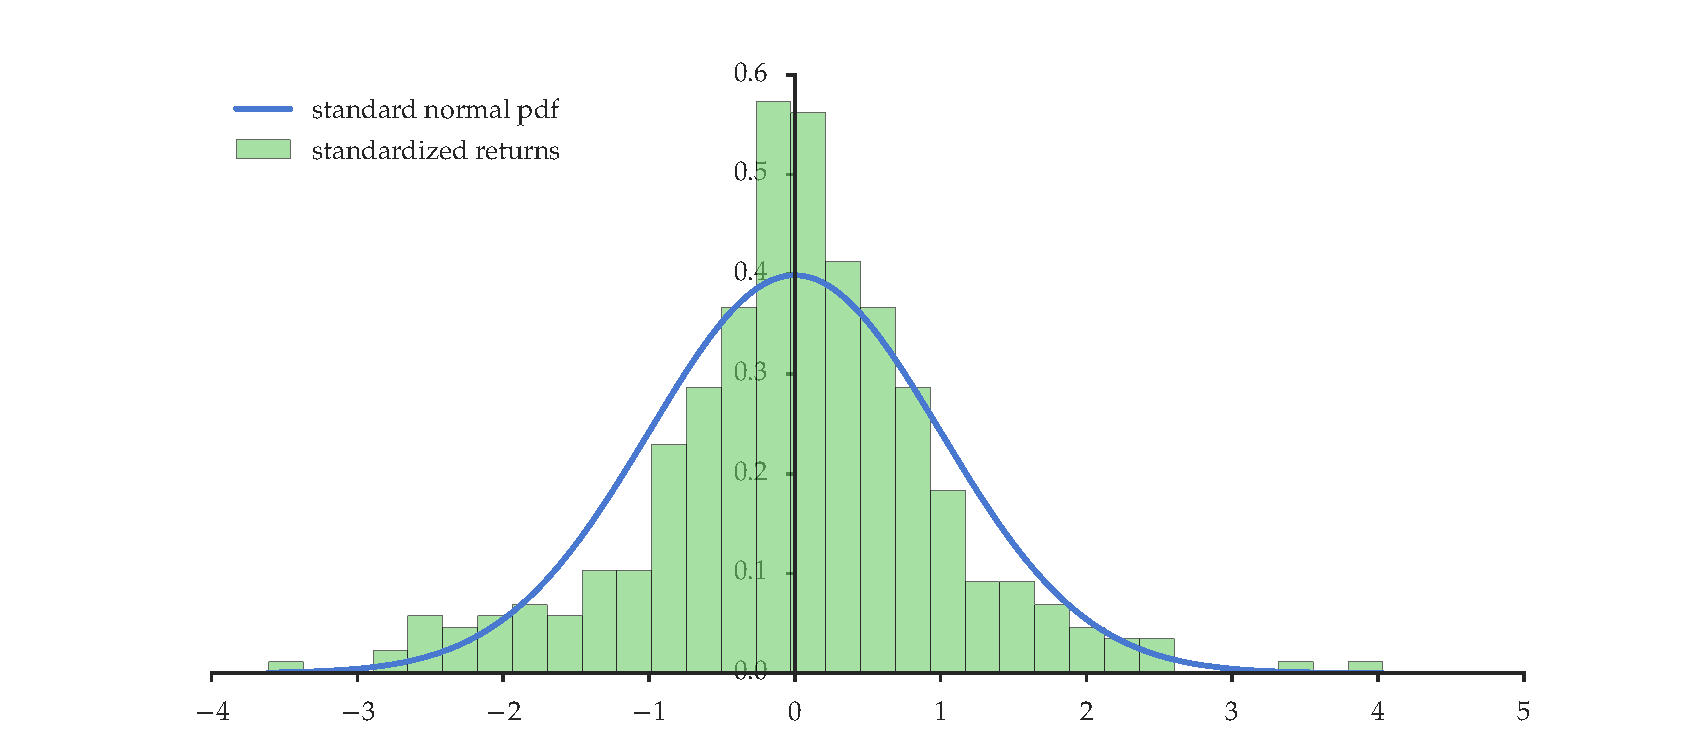
\includegraphics[trim={4em 4em 4em 4em}, clip]{nikkei_hist.pdf}}
    \caption{\label{f:nikkei_hist} Standardized daily returns for the Nikkei 225}
   \end{center}
    \end{figure}
    
\end{frame}

\begin{frame}\frametitle{P-values}

    \vspace{2em}
    Typically, a test that rejects at size 0.05 will also reject at size 0.1, but
    may not reject at size 0.01
    
    Lower $\alpha$ means less tolerance for type I
    error, and forces the critical value to become larger 
    
    \vspace{.7em}
    The $p$-value is the smallest value of $\alpha$
    at which we can still reject given a test statistic
    
\end{frame}

\begin{frame}

    \vspace{2em}
    The null hypothesis is $H_0 :
    \theta \in \Theta_0$ and, for each $\alpha \in (0,1)$, a test $(T,c(\alpha))$
    of size $\alpha$
    
    Assume $c(\alpha)$ determined to solve 
    %
    \begin{equation*}
        \alpha = \sup_{\theta \in \Theta_0} \PP_{\theta}\{T(\zdata) > c\}
    \end{equation*}
    
    In this setting, the $p$-value of the test defined as
    %
    \begin{equation*}
        p(\zdata) := \inf \setntn{\alpha \in (0,1) \, }{\, c(\alpha) <
        T(\zdata) }
    \end{equation*}
    
    \vspace{.7em}
    When $\alpha \mapsto c(\alpha)$ is continuous, the expression for $p(\zdata)$ 
    reduces to 
    %
    \begin{equation*}
        \label{eq:edp}
        p(\zdata) := \text{ the } \alpha \text{ such that } c(\alpha) =
        T(\zdata) 
    \end{equation*}
    
\end{frame}

\begin{frame}

    \vspace{2em}
    \Eg
    Let $x_1,\ldots,x_N$ be an {\sc iid} sample with mean $\theta$ and variance
    $\sigma^2$
    
    Assume both $\theta$ and $\sigma$ are unknown
    
    We wish to test the hypothesis $H_0 \colon \theta =
    \theta_0$
    
    \vspace{.7em}
    Consider the statistic 
    %
    \begin{equation*}
        \label{eq:easn2}
        t_N 
        := \sqrt{N} \left\{ \frac{\bar x_N - \theta_0}{s_N}  \right\}
        =  \frac{\bar x_N - \theta_0}{\se(\bar x_N)}
    \end{equation*}
    %
    where $\se(\bar x_N) := \frac{s_N}{\sqrt{N}}$
    
    Expression converges in
    distribution to a standard normal
    
\end{frame}

\begin{frame}
    
    \vspace{2em}
    \Eg (cont.)
    Hence
    %
    \begin{equation*}
        \label{eq:easn3}
        \phi_N(\boldx) := \1 \{ |t_N| > z_{\alpha/2} \}
    \end{equation*}
    %
    is asymptotically of size $\alpha$ (see ex.~\ref{ET-ex:nwald} in ET)
    
    To evaluate the $p$-value, $c(\alpha) := \Phi^{-1}(1 - \alpha / 2)$, 
    and $c(\alpha)$ is continuous in $\alpha$, so we can 
    apply the following definition of $p(\zdata)$
    %
    \begin{equation*}
        p(\zdata) := \text{ the } \alpha \text{ such that } c(\alpha) =
        T(\zdata) 
    \end{equation*}
    %
    To solve for $p(\zdata)$, solve
    for $\alpha$ in the expression $$\Phi^{-1}(1 - \alpha/2) =
    |t_N(\zdata)|$$
        
    Rearrange to obtain
    %
    \begin{equation*}
        \label{eq:pvsc}
        p(\zdata) = 2 \Phi(-|t_N(\zdata)|)
    \end{equation*}    

\end{frame}

\begin{frame}\frametitle{Accepting the Null?}
    
    \vspace{2em}
    Failure to reject the null not necessarily evidence in favour of the null
    
    \vspace{.7em}
    Economists discovered that a newly developed test due to
    \cite{dickey1979distribution} did not reject the null hypothesis of a unit
    root for a variety of economic time series
    \begin{itemize}
        \item called into
        question earlier time series methods that assumed trend
        stationarity
        \item The idea that innovations to major economic time series contain a
        permanent component became something like a stylized fact
    \end{itemize}



\end{frame}

\begin{frame}
    
    \vspace{2em}
    Specialisze to unemployment rates 
    \begin{itemize}
        \item unit root hypothesis was associated with the concept of hysteresis
    \end{itemize}
    
    Unit root null can be expressed as the hypothesis $a = 1$ in the AR(1) process
    %
    \begin{equation}
        \label{eq:unemp}
        u_{t+1} = a u_t + b + \epsilon_{t+1}
    \end{equation}
    %
    Here $\{u_t\}$ is unemployment, $a$ and $b$ are parameters and
    $\{\epsilon_t\}$ is a zero-mean innovation
    
\end{frame}

\begin{frame}
    
    \vspace{2em}
    Standard one-sided Dickey--Fuller test of the unit root null:
    %
    \begin{enumerate}
        \item estimate the parameters as $\hat a$ and $\hat b$ by least squares
        \item reject the null if $T (\hat a - 1) < c$, where $c$ is a critical
            value and $T$ is length of the sample
    \end{enumerate}
    
     \cite{dickey1979distribution} showed the
    test statistic converges in distribution under the null and tabulated critical values for
    different test sizes
    
\end{frame}

\begin{frame}
    
    \vspace{2em}
    A number of studies have been unable to reject a unit root null for
    unemployment rate data 
    
    Interpretation?  
    \begin{itemize}
        \item \eqref{eq:unemp} is a good model for the data with $a=1$
        \item Another possibility:
    data generated by another process against which this test has
    little power
    \end{itemize}
    
    The second possibility seems more plausible than the first ---
    employment rates don't diverge
    
\end{frame}

\begin{frame}

    \vspace{2em}
    Adopt a nonlinear model
    \begin{equation}
        \label{eq:unempnl}
        u_{t+1} = h(u_t) + \epsilon_{t+1}
    \end{equation}
    %
    where $h$ is the generalized logistic function
    
    \begin{itemize}
        \item  for unemployment rates in a band between about
                5 and 15, the process exhibits strong persistence
        \item  for values above and below this number the shape of $h$ causes              drift back to the band --- ``equilibrium forces"
    \end{itemize} 
    
\end{frame}

\begin{frame}

    \begin{figure}
    \centering
    \scalebox{.42}{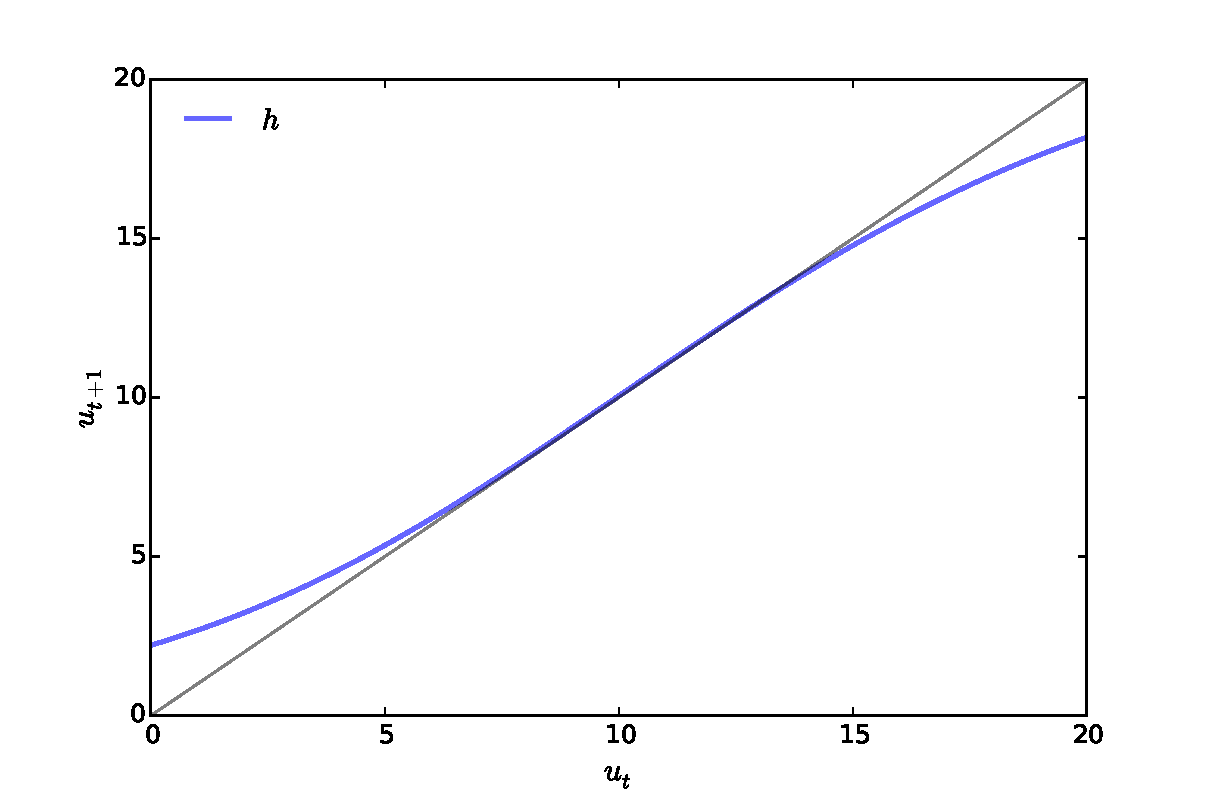
\includegraphics[trim={0em 0em 0em 3em}, clip]{glu.pdf}}
    \caption{\label{f:glu} A nonlinear process for unemployment dynamics}
    \end{figure}

\end{frame}

\begin{frame}

    \begin{figure}
    \centering
    \scalebox{.42}{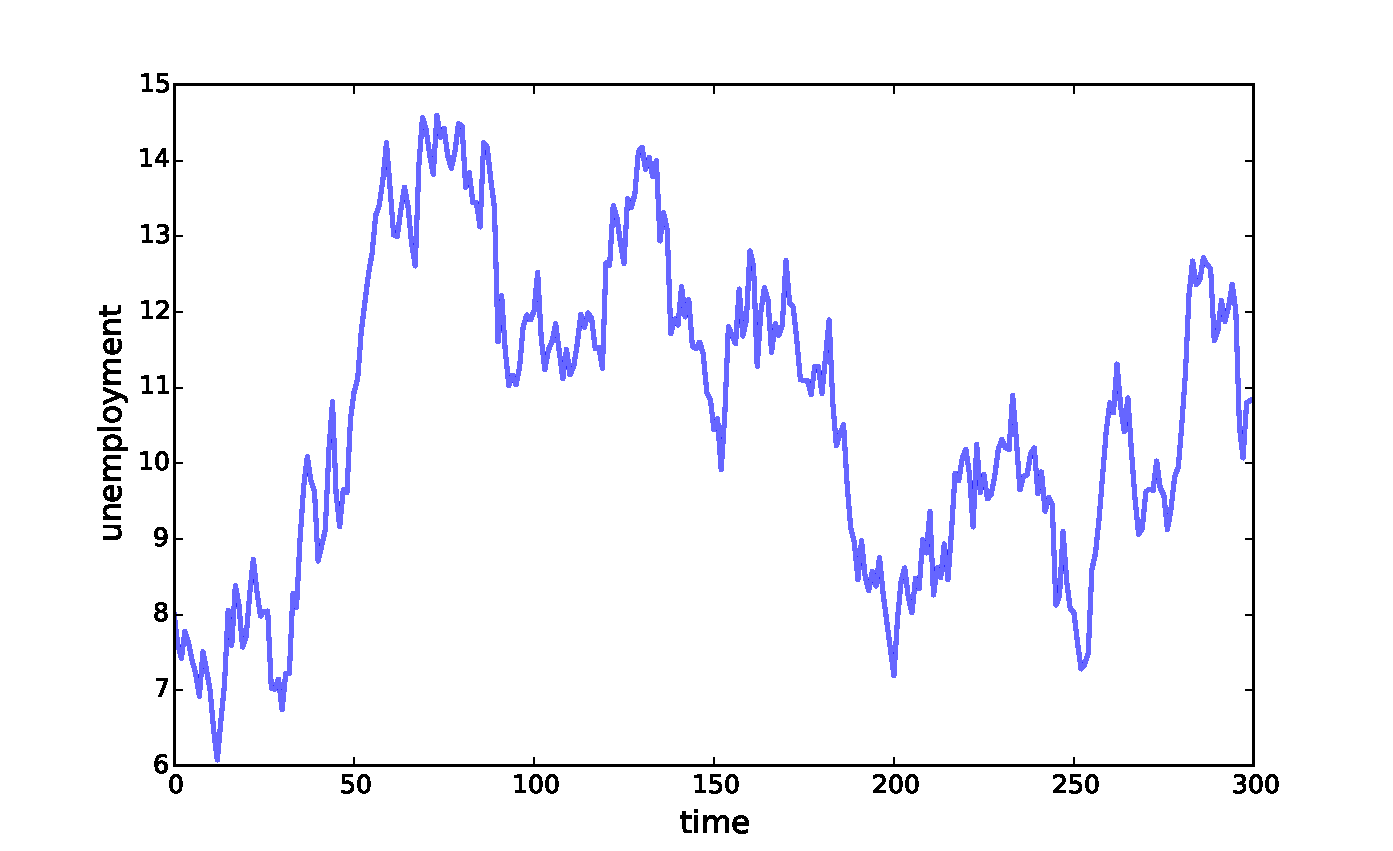
\includegraphics[trim={0em 0em 0em 3em}, clip]{unempl_sim.pdf}}
    \caption{\label{f:unempl_sim} Simulated unemployment dynamics}
    \end{figure}
    
\end{frame}

\begin{frame}

    \vspace{2em}
    Listing~\ref{ET-l:unit_root} in ET gives code for a simulation 
    \begin{itemize}
        \item  shocks $\{\epsilon_t\}$ are independent
        \item time series of length 100 is drawn and the
    Dickey--Fuller test statistic is calculated
        \item  size of the test set to
    0.05
        \item critical value for the test becomes $-13.7$
    \end{itemize}
     
    Rejection frequency over 5,000 repetitions is around
    0.05  -- same rejection frequency as when null is true
    
    \vspace{.7em}
    Yet, nonlinear data-generating process has
    very different properties from the null:  stationary and uniformly ergodic
    
\end{frame}


\end{document}
